\documentclass[dvipdfmx]{jsarticle}

\title{ブロック落しゲーム(JavaScript)}
\author{Seiichi Nukayama}
\date{2020-06-21}
\usepackage{tcolorbox}
\usepackage{color}
\usepackage{listings, plistings}

% Java
\lstset{% 
  frame=single,
  backgroundcolor={\color[gray]{.9}},
  stringstyle={\ttfamily \color[rgb]{0,0,1}},
  commentstyle={\itshape \color[cmyk]{1,0,1,0}},
  identifierstyle={\ttfamily}, 
  keywordstyle={\ttfamily \color[cmyk]{0,1,0,0}},
  basicstyle={\ttfamily},
  breaklines=true,
  xleftmargin=0zw,
  xrightmargin=0zw,
  framerule=.2pt,
  columns=[l]{fullflexible},
  numbers=left,
  stepnumber=1,
  numberstyle={\scriptsize},
  numbersep=1em,
  language={Java},
  lineskip=-0.5zw,
  morecomment={[s][{\color[cmyk]{1,0,0,0}}]{/**}{*/}},
}
%\usepackage[dvipdfmx]{graphicx}
\usepackage{url}
\usepackage[dvipdfmx]{hyperref}
\usepackage{amsmath, amssymb}
\usepackage{itembkbx}
\usepackage{eclbkbox}	% required for `\breakbox' (yatex added)
\usepackage{setspace}
\usepackage{multicol}
\fboxrule=1pt
\parindent=1em
\begin{document}

%% 修正時刻: Sun Jun 21 08:35:35 2020


\section{左右と下の壁を描く}

まず、画面の設定を決めておきます。今回は以下のようにします。

 
 
 
\begin{tcolorbox}
\begin{spacing}{0.5}
\begin{verbatim}
横
20px X 10 = play画面
20px X 1  = 左の壁
20px X 1  = 右の壁

 * 1 2 3 4 5 6 7 8 910 *
+-+-+-+-+-+-+-+-+-+-+-+-+
|*| | | | | | | | | | |*| 0
+-+-+-+-+-+-+-+-+-+-+-+-+
|*| | | | | | | | | | |*| 1
+-+-+-+-+-+-+-+-+-+-+-+-+
|*| | | | | | | | | | |*| 2
+-+-+-+-+-+-+-+-+-+-+-+-+
|*| | | | | | | | | | |*| 3
+-+-+-+-+-+-+-+-+-+-+-+-+
|*| | | | | | | | | | |*| 4
+-+-+-+-+-+-+-+-+-+-+-+-+
|*| | | | | | | | | | |*| 5
+-+-+-+-+-+-+-+-+-+-+-+-+
|*| | | | | | | | | | |*| 6
+-+-+-+-+-+-+-+-+-+-+-+-+
|*| | | | | | | | | | |*| 7
+-+-+-+-+-+-+-+-+-+-+-+-+
|*| | | | | | | | | | |*| 8
+-+-+-+-+-+-+-+-+-+-+-+-+
|*| | | | | | | | | | |*| 9
+-+-+-+-+-+-+-+-+-+-+-+-+
|*| | | | | | | | | | |*| 10
+-+-+-+-+-+-+-+-+-+-+-+-+
|*| | | | | | | | | | |*| 11
+-+-+-+-+-+-+-+-+-+-+-+-+
|*| | | | | | | | | | |*| 12
+-+-+-+-+-+-+-+-+-+-+-+-+
|*| | | | | | | | | | |*| 13
+-+-+-+-+-+-+-+-+-+-+-+-+
|*| | | | | | | | | | |*| 14
+-+-+-+-+-+-+-+-+-+-+-+-+
|*| | | | | | | | | | |*| 15
+-+-+-+-+-+-+-+-+-+-+-+-+
|*| | | | | | | | | | |*| 16
+-+-+-+-+-+-+-+-+-+-+-+-+
|*| | | | | | | | | | |*| 17
+-+-+-+-+-+-+-+-+-+-+-+-+
|*| | | | | | | | | | |*| 18
+-+-+-+-+-+-+-+-+-+-+-+-+
|*| | | | | | | | | | |*| 19
+-+-+-+-+-+-+-+-+-+-+-+-+
|*| | | | | | | | | | |*| 20
+-+-+-+-+-+-+-+-+-+-+-+-+
|*|*|*|*|*|*|*|*|*|*|*|*| 21
+-+-+-+-+-+-+-+-+-+-+-+-+
\end{verbatim}
\end{spacing} 
\end{tcolorbox}




``program.js''を以下のように記述します。

\begin{lstlisting}
 function hajime() {

    // Canvasを取得
    const backgamen = document.getElementById('back');

    const cb =backgamen.getContext('2d');

    // 塗りを設定
    cb.fillStyle = '#CCCCCC';

    // 線を設定
    cb.strokeStyle = '#333333';
    cb.lineWidth = 3;

    // 四角形を塗る
    // cb.fillRect(0, 0, 20, 20);

    // 四角形の枠線を描く
    // cb.strokeRect(0, 0, 20, 20);

    // 左壁を描く
    let x = 0;
    let y = 0;
    let i;

    for (i = 0; i < 22; i++) {
        cb.fillRect(x, y, 20, 20);
        cb.strokeRect(x, y, 20, 20);
        y = y + 20;
    }
	// 右壁を描く
	x = 11 * 20;
	y = 0;
    for (i = 0; i < 22; i++) {
        cb.fillRect(x, y, 20, 20);
        cb.strokeRect(x, y, 20, 20);
        y = y + 20;
    }
	// 下壁を描く
	x = 20;
	y = 21 * 20;
    for (i = 0; i < 20; i++) {
        cb.fillRect(x, y, 20, 20);
        cb.strokeRect(x, y, 20, 20);
        x = x + 20;
    }
}
\end{lstlisting}

この関数を body を読み込んだらすぐに実行させます。
以下のように、\verb!<body>! タグに onload属性で指定しておきます。

\fbox{\textless body onload=''hajime()``\textgreater}

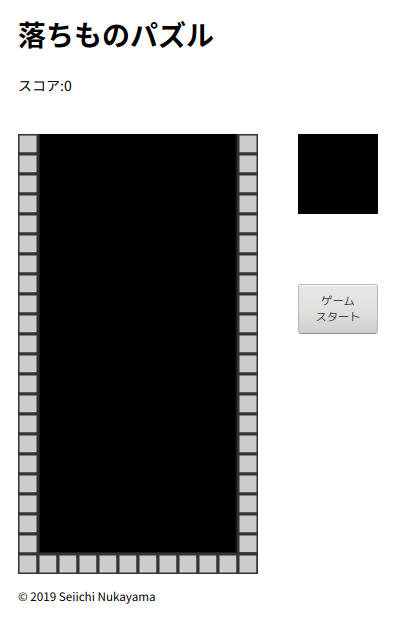
\includegraphics[width=7cm]{game2.png}


\end{document}

%% 修正時刻: Sat May  2 15:10:04 2020


%% 修正時刻: Sun Jun 21 11:41:50 2020
